\chapter{Exemplo}

\section{Tabela com o Pacote Booktabs}

Um exemplo de tabela com o pacote booktabs pode ser visto na Tabela \ref{tabela:exemplo}. A explicação das tabelas sempre vem em cima e esse padrão deve ser respeitado. A numeração é automática e a inserção no índice também. Legal né? \cite{Bennett:QuantumInformationSurvey}

Basta quebrar uma linha para criar um novo parágrafo. Neste parágrafo vou contar que tabelas no \LaTeX dão um pouco de trabalho, mas nada que com paciência não se resolva. Veja os links com dicas que coloquei nos comentários do arquivo \texttt{index.tex}.

\begin{table}[ht!]
\caption{Esta é uma tabela básica em \LaTeX com o pacote booktabs.} \label{tabela:exemplo}
\center{
\begin{tabular}{cccc}
\toprule
Parte 1 & Parte 2 & Parte 3 & Parte 4\\
\midrule
0,415 & 1,365 & 1,98 & 2,05\\
1,36  & 45,5  & 7,98 & 3,01\\
2,36  & 1,35  & 0,15 & 5,32\\
\bottomrule
\end{tabular}}
\end{table}



\section{Inserção de Figuras}

Você pode inserir figuras JPG no \LaTeX! Veja o caso da Figura \ref{fig:exemplo}. Se você quiser outras configurações e dicas, veja o seguinte endereço: \url{http://en.wikibooks.org/wiki/LaTeX/Floats,_Figures_and_Captions}.

A explicação da figura sempre vem embaixo da mesma. Isto aqui é um novo parágrafo apenas para ilustrar a idéia geral de como escrever.

\begin{figure}[H]
\centering
\caption{Um exemplo de figura JPG inserida no \LaTeX.} \label{fig:exemplo}
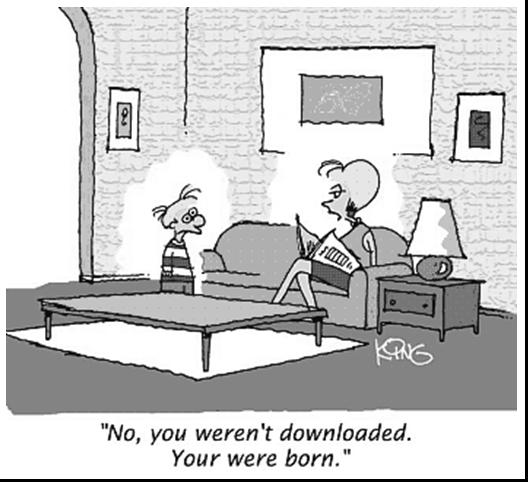
\includegraphics[width=0.4\textwidth]{./img/exemplo.jpg}\\
\small{Elaborado pelo autor.}
\end{figure}

Pode inserir várias figuras lado a lado também. Um exemplo está reproduzido a seguir.

\begin{figure}[H]
  \centering
  \caption{Canal clássico cuja obtenção da capacidade erro-zero é não-trivial.}
  \subfloat[\ ]{\label{fig:exG5}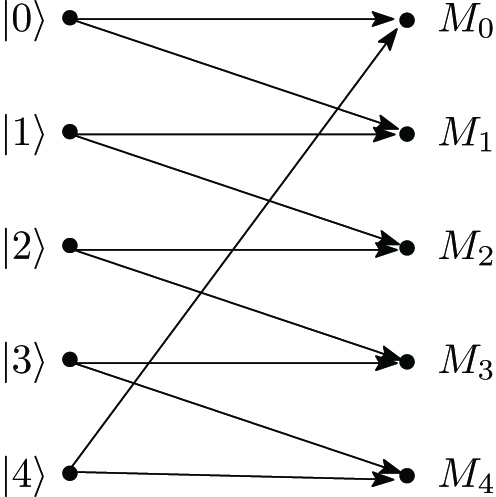
\includegraphics[width=0.3\textwidth]{./img/001}}
  \hspace{0.5cm}
  \subfloat[\ ]{\label{fig:exG52}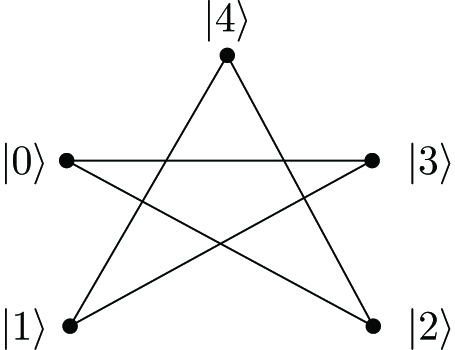
\includegraphics[width=0.3\textwidth]{./img/002}}
  \hspace{0.5cm}
  \subfloat[\ ]{\label{fig:exG53}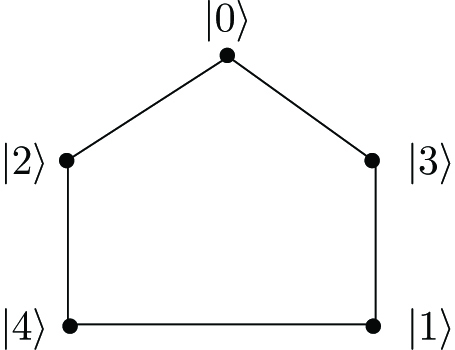
\includegraphics[width=0.3\textwidth]{./img/003}}\\
  \small{Elaborado por Bacon}
\end{figure}

\section{Referências Bibliográficas no Padrão ABNT}

Para gerar versões corretas do \textsc{Bib}\TeX das suas referências, recomenda-se usar o DOI no caso de artigos e o ISBN no caso de livros. Em posse dessas informações, consulte os seguintes links:

\begin{enumerate}
    \item \url{https://www.bibtex.com/c/doi-to-bibtex-converter/}
    \item \url{https://www.bibtex.com/c/isbn-to-bibtex-converter/}
    \item \url{http://doi-to-bibtex-converter.herokuapp.com/}
    \item \url{https://www.doi2bib.org/}
\end{enumerate}

Para saber mais sobre os tipos de referências \textsc{Bib}\TeX e seus significados, consultar a documentação oficial em \url{https://www.bibtex.com/e/entry-types/}.

Este template está integrado com o pacote \texttt{abnt2cite} que produz as referências no padrão ABNT NBR 6023.
